\section{Центр скоростей. Центроиды. Теорема Пуансо}

\subsection{Мгновенный центр скоростей}

\begin{theorem}
  При всяком непоступательном движении плоской фигуры существует точка фигуры,
  скорость которой в данный момент равна нулю.
\end{theorem}

\begin{proof}
  \begin{figure}[H]
    \centering
    \resizebox{\linewidth}{!}{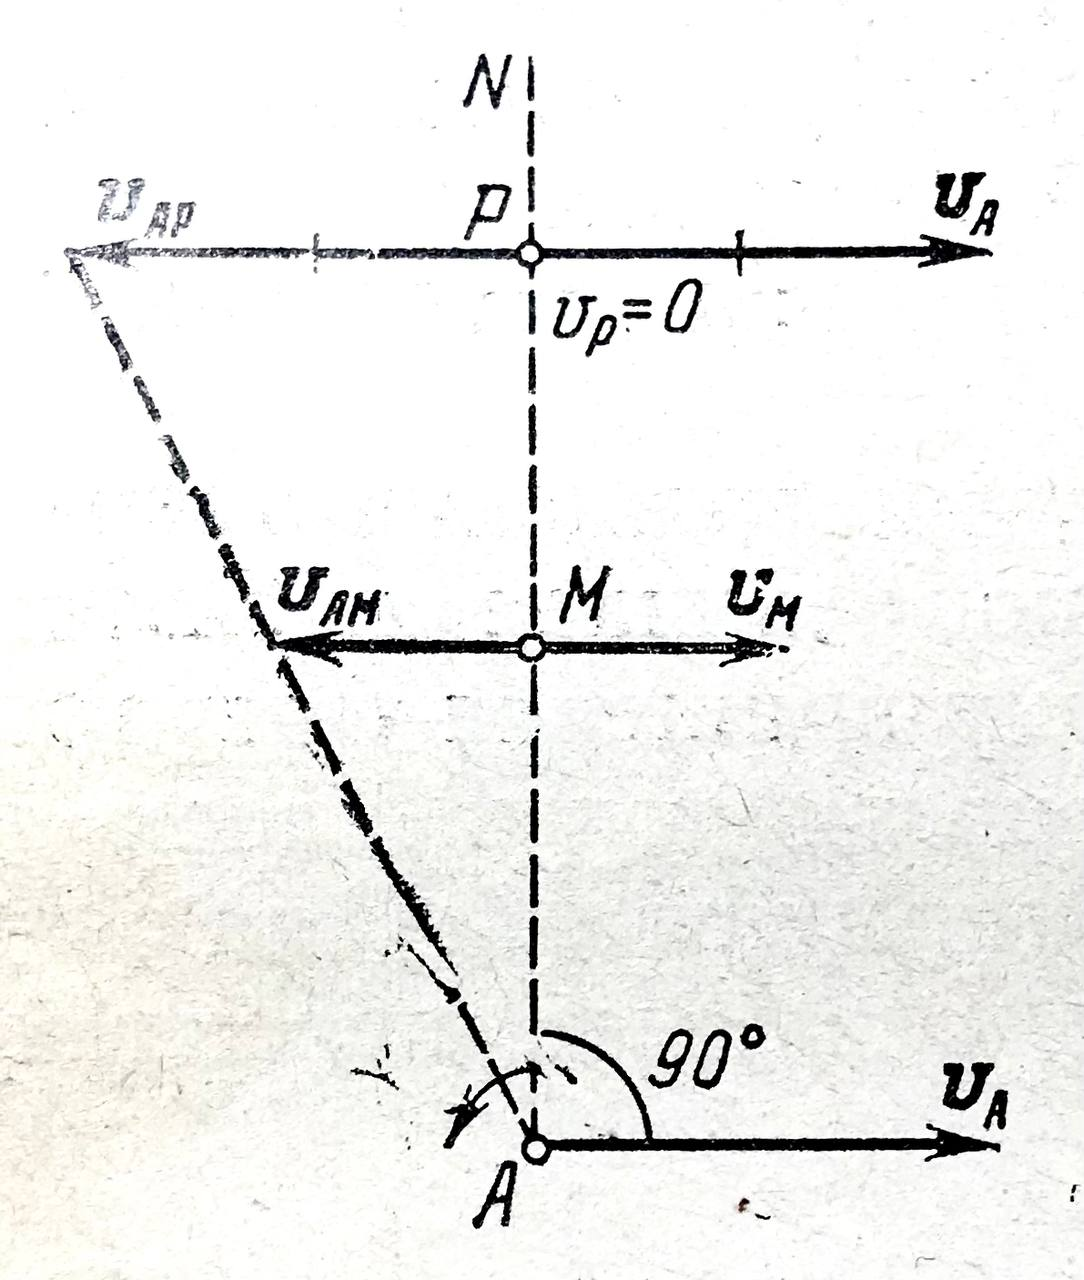
\includegraphics{src/mechanics/pictures/17_1.jpg}}

    \caption{}
    \label{fig:17_1}
  \end{figure}

  Для доказательства восставим из точки $A$ плоской фигуры перпендикуляр $AN$ к
  направлению скорости $\vec{v}_A$ так, чтобы угол $\frac{\pi}{2}$ между
  $\vec{v}_A$ и линией $AN$ был отсчитан в сторону вращения фигуры. Тогда по
  предыдущему вектор скорости любой точки $M$ на этом перпендикуляре будет равен
  \begin{equation*}
    \vec{v}_M = \vec{v}_A + \crossprod{\vec{\omega}}{\vv{AM}} = \vec{v}_A +
      \vec{v}_{AM},
  \end{equation*}
  а величина скорости
  \begin{equation*}
    v_M = v_A - \omega \cdot AM.
  \end{equation*}

  Изменяя расстояние точки $M$ от точки $A$, можно при $\omega \neq 0$ найти
  такую точку $P$, чтобы $v_{AP} = -v_A$; тогда
  \begin{equation*}
    AP = \frac{v_A}{\omega};
  \end{equation*}
  при этом будем иметь
  \begin{equation*}
    v_P = v_A - \omega \cdot AP = v_A - \omega \cdot \frac{v_A}{\omega} = 0.
  \end{equation*}
\end{proof}

\begin{definition}
  Точка $P$ плоской фигуры, скорость которой в данный момент времени равна нулю,
  называется \textit{мгновенным центром скоростей фигуры}.
\end{definition}

Скорости точек плоской фигуры можно рассматривать как вращательные скорости их
вокруг мгновенного центра скоростей, а сам мгновенный центр скоростей --- как
мгновенный центр вращения плоской фигуры.

Имея это в виду, при известных направлениях скоростей точек $A$ и $B$, проведём
через них прямые $l_A$ и $l_B$, ортогональные векторам скоростей в этих точках.
Эти прямые либо пересекаются, либо нет; рассмотрим возможные варианты.
\begin{enumerate}
  \item Прямые $l_A$ и $l_B$ пересекаются в единственной точке --- это и будет
    центр скоростей $P$.

  \item Закреплённые векторы $(A, \vec{v}_A)$ и $(B, \vec{v}_B)$ параллельны,
    направлены в разные стороны или направлены в одну сторону, но не равны по
    величине --- в этом случае прямые $l_A$ и $l_B$ совпадают; через концы
    рассматриваемых закреплённых векторов проведём прямую $l$, --- точка
    пересечения этой прямой с прямой $l_A$ и будет центром скоростей $P$.

  \item Закреплённые векторы параллельны, направлены в одну сторону и равны по
    величине --- в этом случае движение твёрдого тела поступательное, и для него
    понятие центра скоростей не определено.
\end{enumerate}

\subsection{Центроиды}

\begin{definition}
  Траектория мгновенного центра скоростей в плоскости, связанной с движущейся
  фигурой, образует кривую, называемую \textit{подвижной центроидой}.
\end{definition}

\begin{definition}
  Траектория мгновенного центра скоростей в неподвижной плоскости называется
  \textit{неподвижной центроидой}.
\end{definition}

Для вывода уравнений центроид обратимся к формуле \ref{eq:figure_velocity}.
Проектируя её на неподвижные оси $Ox$ и $Oy$, получим
\begin{equation}
  \label{eq:velocity_immovable_projection}
  v_x = v_{0x} - \tilde{\omega} (y - y_0), \quad
  v_y = v_{0y} + \tilde{\omega} (x - x_0);
\end{equation}
проекция же на оси подвижной системы $O'x'y'$ даст
\begin{equation}
  \label{eq:velocity_movable_projection}
  \begin{aligned}
    v_{x'} &= v_{0x'} - \tilde{\omega} y' = \phantom{-}v_{0x} \cos\varphi +
      v_{0y} \sin\varphi - \tilde{\omega} y', \\
    v_{y'} &= v_{0y'} + \tilde{\omega} x' = -v_{0x} \sin\varphi + v_{0y}
      \cos\varphi + \tilde{\omega} x'.
  \end{aligned}
\end{equation}

Подставив в правые части \ref{eq:velocity_immovable_projection} вместо $x$ и
$y$ координаты мгновенного центра скоростей $x_P$ и $y_P$, приравняем левые
части нулю, так как скорость той точки фигуры, которая в данный момент времени
играет роль мгновенного центра, равна нулю. Будем иметь уравнения
\begin{equation*}
  v_{0x} - \tilde{\omega} (y_P - y_0) = 0, \quad
  v_{0y} + \tilde{\omega} (x_P - x_0) = 0,
\end{equation*}
откуда найдём \textit{уравнения неподвижной центроиды}
\begin{equation}
  \label{eq:immovable_centroid}
  x_P = x_0 - \frac{v_{0y}}{\tilde{\omega}}, \quad
  y_P = y_0 + \frac{v_{0x}}{\tilde{\omega}}.
\end{equation}

Аналогично по \ref{eq:velocity_movable_projection} найдём \textit{уравнения
подвижной центроиды}:
\begin{equation}
  \label{eq:movable_centroid}
  \begin{aligned}
    x_P' &= \frac{1}{\tilde{\omega}} \paren{v_{0x} \sin\varphi - v_{0y}
      \cos\varphi}, \\
    y_P' &= \frac{1}{\tilde{\omega}} \paren{v_{0x} \cos\varphi + v_{0y}
      \sin\varphi}.
  \end{aligned}
\end{equation}

\begin{theorem}[Пуансо]
  При плоском непоступательном движении твёрдого тела подвижная центроида
  катится без скольжения по неподвижной.
\end{theorem}

% TODO
(\textcolor{red}{TODO:} доказательство (книга, стр 249))

\subsection{Список литературы}
\begin{enumerate}
  \item \cite{lectures}
  \item \cite{lourie}
\end{enumerate}

